\chapter{Introduction and Review}

This chapter describes the different kinds of biological input data by taking a focus on the biological background of an experimental data set regarding protein-protein interaction of growth factor induced transcriptional signal pathways for inferring regulatory networks. The type of input data and its experimental data collection decides about the choice of an inference model and its interpretation.\\

Afterwards, biological data is put into a graph-theoretical context of a Boolean network. Additionally, this part shows how to capture the dynamics and structural properties of a Boolean network.

\section{Motivation}
%Biological motivation  
The development and functioning of a cell and its organism is a product of a complex cellular machinery, where the interaction of genes, proteins, \gls{mRNA} (messenger RiboNucleotide Acid) and metabolic substances take place in a cascade of extracellular signals transduced by mechanisms of the cell membrane, reaching the nucleus of the cell, initiating a transcription process that controls the production and abundance of proteins. Proper functioning of these regulatory networks is essential to the survival and adaptation of a cell. Malfunctioning has been identified as the cause of various diseases \citep{Berestovsky.2013}.
\\\\
Recent advances in high-throughput techniques provide a big abundance of information about various biological interaction measured over a series of time. It is necessary to handle this big data properly for significant structural and dynamic analysis. Therefore, experimental data is converted into a network structure, where a substance is represented by a node and an interaction is represented by an edge. Mostly substances are part of a big and highly interconnected system where the kinetic information is rarely known \citep{Saadatpour.2013}. Thus, the overall problem of inferring a regulatory network from biological time-course data is to find a trade-off between simplicity, scalability and explanatory power of a network, such that the main important components of a malfunctioning system can be identified for creating medical solutions \citep{Berestovsky.2013} \citep{Barman.2017}.
\\\\
%Different inference approaches of inference
Several models are known of inferring a network from time-course data, which are characterized being either continuous like Ordinary Differential Equation (ODE) models, Baysian models or discrete like Boolean networks (BN)\citep{Saadatpour.2013}. 
%Artificial Neural networks gather their knowledge by detecting patterns and relationships in data and learn through experience. An ANN is constructed by weighted processing elements which constitute the neural layers and are organized in layers. Thus the behaviour of a ANN is determined by a transition function of each variable (neuron), by a learning rule and by the architecture itself. A big advantage, no previous knowledge is needed %\citep{AGATONOVICKUSTRIN2000717}.\\

%Ordinary Differential Equations model
An Ordinary Differential Equation (ODE) creates networks considering kinetic properties of a biological system. This model is a powerful and flexible model to describe complex relations among substances. But kinetic information are rarly available, such that ODE is only a sufficient strategy when a small well known system is analyzed \citep{Saadatpour.2013}.
%\citep{}

%Baysian model
A Bayesian model is a graph-based model of joint multivariate probability distributions that captures properties of conditional independence between variables \citep{Friedman.2000}.\\\\

%Boolean model(BN)
Boolean network models are well known and do not need any kinetic information of a system. Hence, this model simplifies the representation of a complex system, while capturing the main structure and dynamics as well as the steady-state behaviour \citep{Berestovsky.2013}\citep{Saadatpour.2013}. Experimental settings are often financially expensive, such that the time course data sets are quite small. Boolean networks are known being able to derive relationships among substances from relatively small data sets (e.g. 50 measurements for one substance) \citep{Berestovsky.2013}. For this reason the Boolean network model is chosen in this thesis.
%What is a Boolean Network model?
In a Boolean network model, the initial state of a node is either true ($1$) or false ($0$) and the next state is updated according to a Boolean rule  composed by other nodes affecting the nodes state. Updating a nodes' state represents the measurement of sample points over a series of time, such that Boolean trajectories of the model are generated.
\\\\
In general, a pipeline for inferring Boolean networks starts with a normalized time-course data set, which is preprocessed by discretisizing continous values into binary values and remove redundant information. Subsequently,  an inference algorithm learns Boolean rules for each node from the data resulting in a set of rules. The predicted model is tested on itself and the predicted network is scored against a gold standard network.  
\\\\
This work is divided up into two parts for each a pipeline is implemented (available on Git: 'github.com/ninakersten/Masterthesis'). In the first part Boolean networks are learned from \textit{in silico} data sets of \textit{E.coli} and the mammilian cell cycle by three well known inference algorithms Best-Fit, Full-Fit and Reveal \citep{Barman.2017}. The predicted networks are scored against a gold standard, testing the inference algorithms and binarization algorithms on several parameters. 
%Gegen gold standard testen heißt: Predictive power zu ermitteln
%Wie kann die Güte beurteilt werden?Welche metriken gibt es?Wie vergleiche ich die netzwerke?
In the second part results about the algorithms' performance of the first part are taken into account for inferring a real-life time course data set of phophoprotein abundance measurements in breast cancer cell lines (Figure 1.1). This data is provided by the Reverse Engineering Assessment and Methods (DREAM)-Challenge platform. The DREAM-Challenge is a non-profit, collaborative community effort consisting of participants from across the research spectrum of questions in biology and medicine. On this platform real-life data is provided to everyone, such that everyone can participate by contributing own solutions and compare them to other researchers \citep{aboutdream, Bender.2016}.
    
\begin{figure}[H]
\captionsetup{width=0.9\linewidth}
\centering
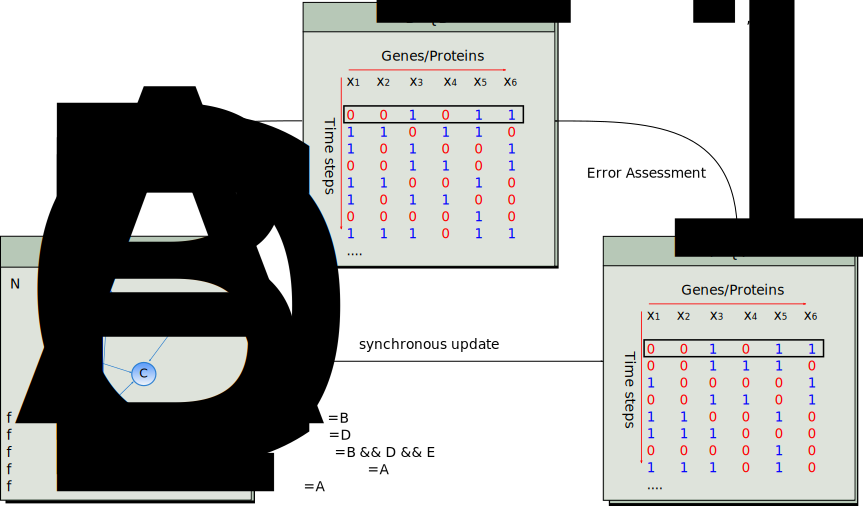
\includegraphics[width=0.8\textwidth]{./Bilder/motivation_pipeline.pdf}
\caption[Raw pipeline]{\textbf{Raw Pipeline.}Continuous input data of either E.coli, the cell cycle or of phosphoprotein interaction in breast cancer cell lines are binarized and redundant data is removed. A network is learned from an inference algorithm (e.g.: \textit{Best-Fit, Full-Fit, Reveal}), its predictive power is evaluated by scoring the output against a gold standard network. }
\label{fig:General Pipeline}
\end{figure} 

This thesis aims to show that a Boolean approach might be a sufficient strategy for inferring big real-life time course data sets by capturing the structure and dynamical properties of a system while emphasizing the limitations which might occur.


\newpage
\section{Biological Background}
%3 Levels of input data
Biological interaction can be observed at different levels of information integration of a cell regarding metabolic interaction, gene-gene interaction and protein-protein interaction.\\ 
%Signal integration
Information integration starts with a signal, which binds to a membrane integrated receptor of the cell causing an activation of one or multiple target proteins inducing several signal transduction cascades (Figure 2.1). While the signal is transduced, it is amplified by enzymatic activities or inhibited by feedback pathways down the cascade. Finally transcription factors are activated by the input signal, such that the expression of a target gene by generating mRNA results in a protein. The resulting proteins influence the cell's survival by its proliferation, induction of cell differentiation and apoptosis.


\begin{figure}[H]
%\setlength{\abovecaptionskip}{0pt}
\captionsetup{width=1.0\linewidth}
\centering
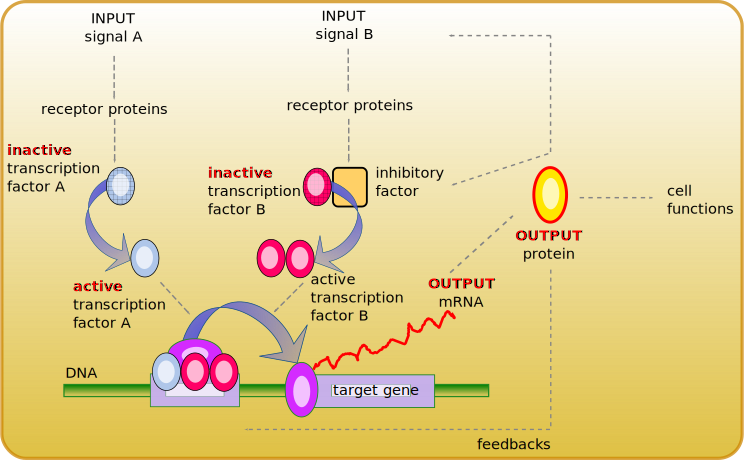
\includegraphics[width=0.85\textwidth]{./Bilder/GRN.pdf}
%\setlength{\abovecaptionskip}{-5ex}
\caption[Transcriptional Signal Cascade]{\textbf{Transcriptional Signal Cascade}
Two different input signals $A$ and $B$ bind to a specific receptor protein. The complex of $A$ activates the transcription factor $A$ that binds directly to the gene's regulatory sequence inducing the expression of the target gene. Different to $A$ initiates the complex of $B$ a separation of the inactive $B$ (\textit{pink oval}) from an inhibitory factor (\textit{yellow rectangle}). Transcription factor $B$ is then free to bind to the cis-regulatory sequence. Thus the expression level of this target gene is leveled by signal $A$ and $B$. The mRNA output results in a protein product which can take place in several processes of the cell \citep{U.S.DepartmentofEnergyOfficeofScience.April2001}.}
%\setlength{\belowcaptionskip}{0pt} 
\label{fig:Fig.2.}
\end{figure}


The concentration of substances in signalling pathways underlies high fluctuation over time due to transcriptional and translational regulation, such that the inference of a significant network is a challenging task \citep{Kestler.2008, Oates.2012}.

\subsection*{Metabolic network}

At the level of metabolic networks the substances are highly interconnected in a quite complex way (e.g. cell respiration in Figure 1.3). An individual's metabolism is determined by its genetics, environment and nutrition.\citep{Shmulevich.2002}. In a metabolic network the nodes are depicted by different types of biochemical components connected by directed edges describing a activating or inactivating interaction. Biochemical reaction are represented by a metabolic pathway, which consists of a sequence of biochemical reactions that produce a set of metabolites from a set of precursor metabolites and cofactors. The length of a pathway is the number of biochemical reactions between the precursor and the final metabolites of the pathway \citep{Shmulevich.2003}. 
%The definition of a pathway is not unique, therefore the length of pathways vary. 

\begin{SCfigure}[][!h]
%\centering
%\captionsetup{width=.7\linewidth}
\begin{minipage}{0.65\linewidth}
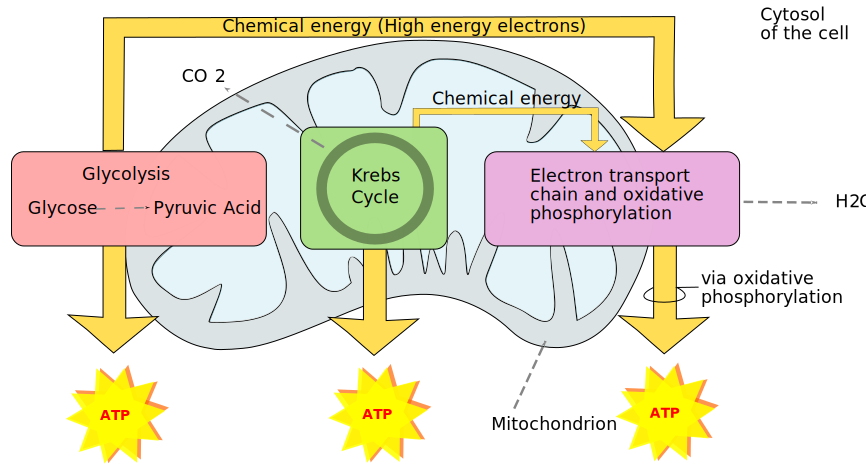
\includegraphics[width=1.0\textwidth]{./Bilder/metabolic.pdf}
\end{minipage}
%\begin{minipage}{width=0.3\textwidth}
\caption[Metabolic Network for cell respiration]{\textbf{Metabolic Network for cell respiration. } In a mitochondrion, an essentiell compartment of the cell, converts energy derived from nutrition into biochemical energy \gls{ATP}(Adenosin TriPhosphate) by releasing waste products of water $H_{2}O$ and $CO_{2}$.}
%\end{minipage}
\label{fig:Fig.3.}
\end{SCfigure} 
\citep{cellrespiration}


\subsection*{Gene regulatory network}

In a gene regulatory network (\gls{GRN}) depicted in Figure 1.2 the interaction of genes are identified indirectly by the abundance measurement of their transcriptional products (e.g. mRNA, proteins). The nodes of a GRN are depicted by the genes' names and the edges are directed by showing whether a gene produces proteins which inhibit or activate a target gene  \citep{Karlebach.2008}.



%\newpage
\subsection*{Protein-Protein-Interaction network}
In contrast to the gene regulatory interaction network in a protein-protein interaction (\gls{PPI}) network the proteins act directly among themselve. Thus the nodes in a network are the interacting proteins. Proteins interact by physical contacts (e.g. electrostatic forces) of high specificity. PPIs play a big role in electron transfer, signal transduction, transport across the membrane and cell metabolism. The underlying assumption is that true interactions are likely to occur between proteins involved in the same biological process, proteins found in the same cell compartment, and proteins whose mRNA are co-expressed \citep{LasRivas.2010}\citep{Pellegrini.2004}.\\

The real-life data set of the DREAM-Challenge used in this work is dealing with PPIs, thus, it is important to know for later data collection, data processing and discussion how the data is obtained and which role these PPIs play in a biological context.\\

Referring to the general description of a transcriptional signal cascade (Figure 1.2) we state the receptor being an enzyme-associated receptor and the input signals are growth factors. An enzyme associated receptor has a polypeptide chain integrated in the cell's membrane with a tyrosine kinase activity (Figure 1.4).


\begin{figure}[H]
%\setlength{\abovecaptionskip}{0pt}
\captionsetup{width=.9\linewidth}
\centering
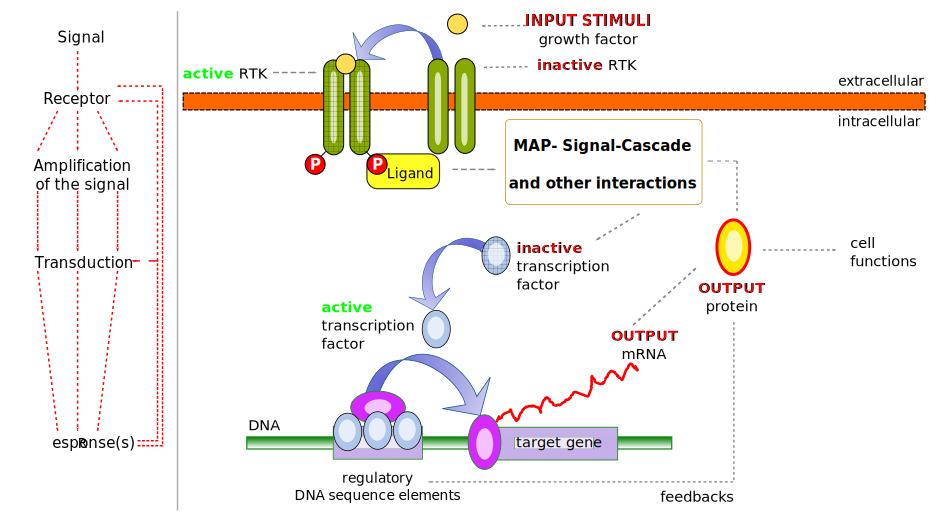
\includegraphics[width=0.8\textwidth]{./Bilder/GRNDREAM8.pdf}
%\setlength{\abovecaptionskip}{-5ex}
\caption[Transcriptional Signale Cascade of RTKs]{\textbf{Transcriptional Signale Cascade} An incoming stimuli (\textit{yellow circle}) representing a growth factor binds to an inactive RTK (\textit{green}), such that the RTK is activated. The RTK amplifies the signal and initiates a signal transduction cascade, such that an inactive transcription factor (\textit{blue oval}) is activated, which binds to regulatory DNA sequence elements inducing the mRNA transcription of a target gene resulting in a new protein \citep{U.S.DepartmentofEnergyOfficeofScience.April2001}. }
%\setlength{\belowcaptionskip}{0pt} 
\label{fig:DREAM8GRN}
\end{figure}


Growth factor receptors with a tyrosine kinase activity are called receptor tyrosine kinases (\gls{RTK}s). These RTKs have the property of autophosphorylation, meaning that they amplify their incoming signal. Binds a ligand to this receptor, first the receptor autophosphorylates and then phosphorylates the tyrosin residues of the ligand. By the phosphorylation of the receptor and several other ligands (resp. proteins) a phosphorylating cascade (e.g. signal transduction cascade) is induced. In this mitogen activated protein (MAP) phosphorylation cascade the \gls{MAP}-kinase katalyzes the phosphorylation of effector proteins, such that inactive transcription factors are activated starting the transcription process of a target gene and finally resulting in a protein product \citep{MullerEsterl.2009}.\\

\newpage
In the DREAM-Challenge growth factors are selected depicted as a stimuli by pertubating the cell's signal transduction. Thus, different stimuli cause different signal transduction cascades. Depending on the incoming stimuli particular proteins take place in the signal transduction cascade. The goal is to figure out PPIs in this phosphorylation cascade by inferring a Boolean network based on the measurement of the proteins abundance considering eight different incoming growth factors (resp. stimuli) displayed in Table 1.1. 
dysregulation of the genes of these growth factors have been linked to diseases such as cancer, schizophrenia, bipolar disorder and many more \citep{NRG1}.


%{\tabcolsep=2.5pt%
\begin{center}
\captionsetup{width=0.87\linewidth}
%\setlength\extrarowheight{4pt}
%\noindent\begin{tabular}{c|c|l}
%\def\arraystretch{2.0}%
\scriptsize
%\addtolength{\tabcolsep}{-5pt}
\begin{tabular}{lll}
\toprule 
 Notation & Name & Description\\
\hline\hline
IGF1 & Insulin like Growth Factor 1 & \parbox{8cm}{Hormone, similar to the insulin function and structure \citep{IGF1}}\\
\midrule NRG1 & Neuregulin 1 & \parbox{8cm}{Membrane glycoprotein, mediating cell-cell signalling, critical role in growth and developement of the cell \citep{NRG1}}\\
\midrule HGF & Hepatocyte Growth Factor & \parbox{8cm}{Regulate cell growth, cell motility and morphogenesis \citep{HGF}} \\
\midrule FGF1 & Fibroblast Growth Factor 1 & \parbox{8cm}{Functions as a modifier of endothelial cell migration, proliferation and an angiogenic factor\citep{FGF1}}\\
\midrule Insulin & Insulin & \parbox{8cm}{Mutations in this gene are associated with type II diabetes and susceptibility to insulin resistance \citep{Insulin}}\\
\midrule EGF & Epidermal Growth Factor & \parbox{8cm}{This protein acts a potent mitogenic factor that plays an important role in the growth, proliferation and differentiation of numerous cell types \citep{EGF}.}\\
\midrule PBS & Translocator Protein (TSPO) &  \parbox{8cm}{Present mainly in the mitochondrial compartment of peripheral tissues. The protein is a key factor in the flow of cholesterol into mitochondria to permit the initiation of steroid hormone synthesis \citep{PBS} \citep{PBS}.}\\
\midrule Serum & SRF & \parbox{8cm}{Member of the MADS box superfamily
of transcription factors \citep{Serum}}\\
\bottomrule
\end{tabular}
\captionof{table}{List of growth factors (stimuli) of DREAM8 Challenge}
%List of growth factors (resp. hormons) used in the Dream8 Challenge. All of them take place in the regulation of the cell's functions. Malfunctioning of these signals may cause several diseases (e.g. cancer).}
\end{center}
%}


%\newpage
%RPMA vllt. besser in den Teil: Data collection of DREAM8-Challenge packen?
\subsubsection*{Reverse phase Protein lysate MicroArray}
One of the most effetive strategy to collect data of protein-protein interaction is a technique so called reverse phase protein lysate microarray(\gls{RPMA}, resp. RPPA). RPMA is an antibody-based assay that provides quanitative measurements of protein abundance \citep{authornamenotavailable.}.
This technique is divided up into 6 parts. First starting with the sample collection. An inhibitor or stimulus in form of drugs is added to a set of cell lines at the same time and the cell lines are then processed at different time points. Secondly in the cell lyses step cell fragments are lysed with a cell lysis buffer to obtain high protein concentration. The choice of a buffer decides the quantity of proteins that can be lysed out of the cell. Afterwards cell lysed probes are diluted. In the Antibody screening the lysates are pooled and resolved by \gls{SDS-PAGE} (Sodium Dodecyl Sulfate - Polyacrylamide Gel Electrophoresis) followed by western blotting on a nitrocellulose membrane \citep{AlTubuly.2000}. The membrane is cut into 4mmm strips. Each slide is probed with a different antibody, where a primary antibody is extended by a secondary antibody. For fluorometric detection primary and secondary antibody are diluted (Figure 1.5). %A detection reagent is put on each slide. Signal amplification and detection is done by an optical flatbed scanner if colormetric technique is used or by laser scanning. 
The resulting data is normalized, such that outliers are excluded from the data's structure \citep{Boellner.2015}.\\

\begin{SCfigure}[][!h]
	%\setlength{\abovecaptionskip}{0pt}
	%\captionsetup{width=0.7\linewidth}
	%\centering
	\begin{minipage}{0.6\linewidth}
	\includegraphics[width=0.9\textwidth]{./Bilder/RPMA.pdf}
	\end{minipage}
	%\setlength{\abovecaptionskip}{-5ex}
	\caption[RPMA: Antibody binding and fluorometric detection]{\textbf{RPMA: Antibody binding and fluorometric detection.} Proteins are tagged by a specific antibody. After incubation time the secondary antibody is added. Finally the abundance of proteins is determined by a fluorometric detection.}
	%\setlength{\belowcaptionskip}{0pt} 
	\label{fig:Fig.4}
\end{SCfigure}

The strength of RPMA is the high throughput, ulta-sensitive detection of proteins from extremely small numbers of input material which is not possible for western blotting and \gls{ELISA} (Enzymatic Immunoassay) \citep{Boellner.2015}. The small spot size on the microarray, ranging in diameter from 85 to 200 micrometres, enables the analysis of thousands of samples with the same antibody in one experiment \citep{Ramaswamy.2005}. The high sensitivity of RPMA allows for the detection of low abundance proteins or biomarkers such as phosphorylated signaling proteins from very small amounts of starting material such as biopsy samples, which are often contaminated with normal tissue\citep{Sheehan.2005}. A great improvement of RPMAs over traditional forward phase protein arrays is a reduction in the number of antibodies needed to detect a protein \citep{Sheehan.2005, Liotta.2003}. The protein isn't detected directly which helps to preserve the proteins. Antibodies, especially phospho-specific reagents, often detect linear peptide sequences that may be masked due to the three-dimensional conformation of the protein. This problem is overcome with RPMA as the samples can be denatured, revealing any covered epitopes (part of a protein recognized by specific antibody)\citep{Liotta.2003}.\\

The weakness of RPMA are batch effects caused by the choice of the right buffer, quantity of the proteins and the antibody performance.
The choice of the right buffer decides the quantity of proteins which can be lysed out of the cell. Little or poor quality of starting material and a long storage time causes low protein. It might be useful to improve the antibody performance by validating it with a smaller sample size under identical conditions before starting with the actual sample collection. Currently the number of signalling proteins for which antibodies exist to get an analyzable signal is quite small. \\

\newpage
\section{Graph-theoretical Background}
This section is dealing with defining the graph-theoretical properties of a Boolean network $N$ in terms of its structure and dynamics.\\


\begin{defn}
\textbf{Boolean Network}\\
\textit{A Boolean network $N$ is defined by an n-dimensional binary vector $X=(x_{1},...,x_{n})$, where each element $x_{i}\in X$ corresponds to the state $x_{i}=1$ or $x_{i}=0$ of a species $i$. Then a set $F$ of $n$ transition functions contains a particular function $f_{i}$ for each species $x_{i}$ \citep{Berestovsky.2013}. 
Every transition function $f_{i} \in F$ is therefore a n-variable Boolean function $f:\mathbb{B}^{n} \rightarrow \mathbb{B} $, which is represented by a Boolean expression over $n$ input variables \citep{HannesKlarner.November2014}.
\\For every $f_{i}\in F$ s.t. $1\le i\le n$,
\begin{equation}
f_{i}(X(t))=x_{i}(t+1)
\end{equation}
, where $f_{i}(X(t))$ defines the next state for each $x_{i}$ at time $(t+1)$ in the network.}
\end{defn}


In a biological context the activity of a node is a qualitative rate whether a gene is being transcribed $x_{i}=1$ or not $x_{i}=0$, a transcription factor is active or inactive, a protein's concentration is above or below a certain threshold (e.g. phosporylated or un-phosphorylated). Thus a network with $n$ nodes will have $2^{n}$ possible states.
\citep{Saadatpour.2013}\citep{Lahdesmaki.2003}\citep{HannesKlarner.November2014T}.
\\
Then a transition $f_i$ describes a rule of $n$ node defining by their activating or inhibitory influence on a target node the next state of a that node \citep{Berestovsky.2013}.\\

For instance, a gene $x_{A}$ is activated by another gene $x_{B}$ and inhibited by a second gene $x_{C}$. Then the transition function of $x_A$ is $f_{x_{A}}=x_{B} \land  \neg x_{C}$ and the Boolean algebra looks like this;

\hspace{-15px}
\begin{equation}
\begin{split}
x_{A}& = x_{B} \text{ \&\&  !} x_{C} 
\end{split}
\end{equation}

, where a Boolean function is a composition of nodes $x_{i}\in X$ and logical operators represented by '\&\&', '||', '!' (resp. 'NOT', 'AND' and 'OR' ;resp. '$\land$' ,'$\lor$' , '$\neg$') \citep{Saadatpour.2013}\citep{Berestovsky.2013}. \\

A Boolean network can be abstracted into a graphical representation of an interaction graph capturing the structural properties of it. Therefore the notation of a directed graph is introduced.

\newpage
\begin{defn}
\textbf{Directed Graph}\\
\textit{A directed graph $G=(V,A)$ is an ordered pair, defined as a set of nodes $V=\{v_{1},v_{2},...,v_{n}\}$ and a set of directed edges $A$ denoted as 'arcs'. A set of directed edges $A=\{ (i,j)|i,j\in V\} $ describes the flow of information in a network, where $(i,j)$ describes a flow from $i$ (tail) to $j$ (head)} (Figure 1.6).\\
\end{defn} 
\citep{Pavlopoulos.2011}

\begin{defn}\textbf{Interaction Graph}\\
\textit{The interaction graph (\gls{IG}) (resp. dependency raph) of a Boolean network $N$ is a directed graph $IG(X,A)$ that consists of the node set $X$ and the arc set $A = A _{F} \subseteq X \times X$ with $(x_{i},x_{j})\in A \text{ iff }f_{x_{j}}$ depends on $x_{i}$, then:}
\end{defn} 
\begin{equation}
a_{ij}=\begin{cases}
1 & \text{ if there is an edge from node i to node j}\\
0 & \text{ otherwise}
\end{cases}
\end{equation}
\citep{HannesKlarner.November2014T}
%(Gutes Paper mit Definitionen:!!!!!\citep{Pavlopoulos.2011})

\begin{SCfigure}[][!h]
	%\begin{figure}[H]
	\begin{minipage}{0.4\linewidth}
	%\vspace{-\baselineskip}
	%\captionsetup{width=0.7\linewidth}
	\hspace{30px}
	%\centering
	\includegraphics[width=0.5\textwidth]{./Bilder/DirectedGraph.pdf}
	\end{minipage}
	\caption[Directed Graph \textit{G}]{\textbf{Directed Graph \textit{G}. }$a_{i,j}$ is a directed edge (arc) depicting the flow of information from node $i$ to node $j$.}
	\label{fig:7}
\end{SCfigure}
%\end{figure}

In an interaction graph for each node being described by another one, this connection is written '$x_{i}$ $1$ $x_{j}$' and for the case that there is no connection '$x_{i}$ $0$ $x_{j}$', respectively.
\\\\
Furthermore an interaction graph provides information about nodes having a positive or negative influence on other nodes depicted by the \textit{Sign} of an edge. This term is introduced for completion and is not necessary for later investigation in this thesis. 

\begin{defn}\textbf{\textit{Sign} of an edge}\\
\textit{The sign of an edge is defined by $Sign(x_{i}\rightarrow x_{j}) \subseteq \{+,-\}$.}
\end{defn}

Then the expression $x_{i}\rightarrow x_{j}$ is either $x_{i}\xrightarrow{+}  x_{j}$ (resp. $x_{i}$ $1$ $x_{j}$) describing an activating connection, $x_{i}\xrightarrow{-} x_{j}$ (resp. $x_{i}$ $-1$ $x_{j}$ ) describing an inhibitory connection or both $x_{i}\xrightarrow{+,-} x_{j}$ (resp. $x_{i}$ $1,-1$ $x_{j}$ ).\\

\begin{SCfigure}[][!h]
\begin{minipage}{0.4\linewidth}
%\captionsetup{width=0.9\linewidth}
%\vspace{-10px}
%\centering
\includegraphics[width=0.58\textwidth]{./Bilder/Interactiongraph1.pdf}
\end{minipage}
\caption[Interaction graph \textit{G}]{\textbf{Interaction graph \textit{IG}. }Relating to the Boolean rule (1.2) a node $x_{A}$ is activated (\textit{green}) by $x_{B}$ and inhibited (\textit{red}) by $x_{C}$.}
\label{fig:7}
\end{SCfigure}

 
The number of incoming edges of a node denoted by the \textit{\textbf{in-degree}} of a node is a sufficient parameter for complexity analysis in a network. 

\begin{defn}\textbf{\textit{In-degree}}\\
The \textit{in-degree} of a node is the number of incoming edges to a node determining its state.
\begin{equation}
k^{in}_{i}=\sum_{j}{a_{ij}}
\end{equation}
\end{defn}
\citep{Barman.2017, NykampDQ.hiddene}
%(Gutes Paper mit Definitionen:!!!!!\citep{Pavlopoulos.2011})
Hence, the out-degree describes the number of outgoing edges of a node. Nodes with only outgoing edges (in-degree$=0$) are called sources, and nodes with only incoming edges (out-degree$=0$) are sinks of the network. The higher the \textit{in-degree} of a node, the more nodes are part of its transition function $f$ and the complexity increases. Here, the \textit{in-degree} of $x_{A}$ in Figure 1.7 is $k^{in}_{x_{A}}=2$.\\

%It is desireable to determine the nodes whos \textit{in-degree} is the highest among other nodes, whose removal can break down the network into isolated clusters \citep{Albert.2002}. 
%\begin{defn}\textbf{Indegree}\\
%\textit{}
%\end{defn}

Furthermore the dynamics of a system (resp. the state change behaviour of a node over a series of time) can be simulated by repeatedly applying the set $F$ of transition functions to the corresponding set of nodes $X$ and updating their 'current' state \citep{Berestovsky.2013}.\\
In a \textit{\textbf{synchronous}} simulation, the states of all nodes are updated simultaniously after all transition function of $F$ have been applied to all nodes $X$. In contrast to the \textit{\textbf{asynchronous}} simulation, the states are updated by randomly choosing a transition function $f_{i}\in F$ and updating the state of $x_{i}$ in the exact time \citep{Hopfensitz.2012, Liang.1998, Lahdesmaki.2003, Albert.2008}.
In biological processes interaction of substances rarely happen at the same time, thus dynamical analysis is an important factor of detecting interacting substances.
\\\\
These two terms of updating a node's state are abstracted in a so called \textit{state transition graph} \citep{Saadatpour.2013}.

\begin{defn}\textbf{State Transition Graph}\\
\textit{A state transition graph (\gls{STG}) is a directed graph with a set of nodes represented by a set of binary vectors $F(t+1)=\{ f_{1}(X(t+1)),...,f_{n}(X(t+1))\}$, representing the updated states of all variables after all of the functions in $F$ have executed. The arcs denote possible transitions from one binary state vector to another}.
\end{defn}
\citep{Saadatpour.2013, Lee.2002, HannesKlarner.}
%\raggedbottom
\\
Starting from an initial state in the state transition graph and iteratively updating the state of the nodes, the state of the system evolves over time by following a trajectory of states until the nodes' states do not change anymore: $X(t)=X(t+1)$ , so called \textbf{\textit{steady-state}} \citep{Saadatpour.2013, Liang.1998}. These steady-states describe the 'true' state of the nodes in a system, thus the 'true' connection of the nodes to each other. 
\\\\
The following example demonstrates deriving $F$ from an interaction graph $IG$, calculating the corresponding set of binary trajectories $B=\{B_{1},...,B_{n}\}$ (one per species) updated in a synchronous and asynchronous manner resulting in two state transition graphs.
\\\\
\textbf{Example 1.1} The interaction graph in Figure 1.8 shows a Boolean network with three nodes $X=\{x_{1},x_{2},x_{3}\}$ (\textit{blue circle}), where positive (resp. activating) edges (\textit{green}) and negative (resp. inhibiting) edges (\textit{red}) represent the interaction between the nodes. The \textit{in-degree} of $k^{in}_{x_{1}}=2$, $k^{in}_{x_{2}}=1$ and $k^{in}_{x_{3}}=3$.

 
\begin{figure}[H]
\centering
\includegraphics[scale=1.2]{./Bilder/examplenetwork.pdf}
%\end{minipage}
\caption[Interaction Graph]{\textbf{Interaction Graph}}
\label{fig:IG}
\end{figure}
%Graphik und caption an die Breite der seite anpassen


From the interaction graph the set of transition functions $F$ (resp. Boolean functions) can be derived (1.6) such that the state transition graph can be calculated.

\begin{equation}
F(x_{1,2,3}) = 
\begin{pmatrix}
x_1      & \land & x_2 & \land &\neg x_3\\
\neg x_1 &       &      &       & \\
         &       & x_2  &\land & x_3
\end{pmatrix}
\end{equation}


For every possible state of $x_i\in X$ the next state $f_{i}(X(t))=x_{i}(t+1)$ is calculated shown in the computation (1.7)-(1.14) below \citep{Remy.2008}.


\begin{align}
x(t)& =(0,0,0) &\rightarrow & &f(x(t+1)) = (0,1,0)\\
\color{red}x(t)& \color{red}=(0,0,1) &\color{red}\rightarrow & &\color{red}f(x(t+1)) = (0,1,0)\\
x(t)& =(0,1,0) &\rightarrow & &f(x(t+1)) = (0,1,0)\\
x(t)& =(1,0,0) &\rightarrow & &f(x(t+1)) = (0,0,0)\\
x(t)& =(1,1,0) &\rightarrow & &f(x(t+1)) = (1,0,0)\\
\color{red}x(t)& \color{red}=(1,0,1) &\color{red}\rightarrow & &\color{red}f(x(t+1)) = (0,0,0)\\
x(t)& =(0,1,1) &\rightarrow & &f(x(t+1)) = (0,1,1)\\
\color{red}x(t)& \color{red}=(1,1,1) &\color{red}\rightarrow & &\color{red}f(x(t+1)) = (0,0,1)
\end{align}

As we know from the description of asynchronous STG's in biological systems processes happen uncommonly at the same time, which is observed by comparing state transition graph of the synchronous (A) and asynchronous (B) model in Figure 1.9. In contrast to the synchronous STG where each state has a unique successor, in the asynchronous STG multiple successors of a trajectory are possible (e.g. (1.8),(1.12),(1.14)) \citep{Saadatpour.2013}. 

\begin{figure}[H]
  \centering
% \begin{varwidth}{\linewidth}
    \includegraphics[scale=.7]{./Bilder/asynchronexample.pdf}
  %\end{varwidth} % ein Leerzeichen Abstand
  %\begin{varwidth}{\linewidth}
   % \includegraphics[scale=.6]{./Bilder/example01_asynchron_stg}
 % \end{varwidth}
  \caption[Synchronous and Asynchronous State Transition Graph]{\textbf{Synchronous and Asynchronous State Transition Graph}. (A): Synchronous state transition graph; and (B): Asynchronous state transition graph of a Boolean network. Binary digits from left to right depict the state of the nodes $x_1$,$x_2$,$x_3$. The dark gray states are possible steady-states in the system.}
\label{fig:Fig.4.}
\end{figure}


%S (set of states),B(binarized boolean trajectories),k(indegree value),n(number of nodes),m(number of measurements) Begriffe einführen
%\\newpage


